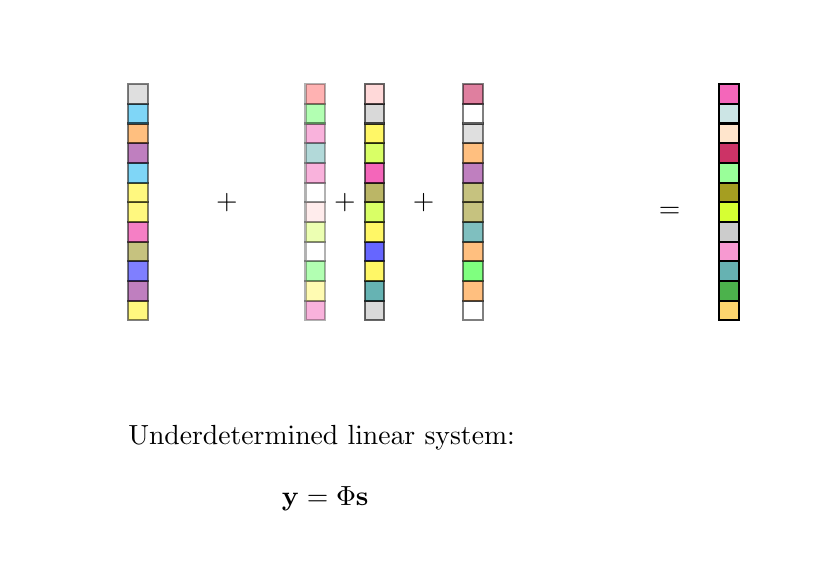
\begin{tikzpicture}
[draw=black, line width=0.75pt,
entry/.style={rectangle, draw, inner sep=0pt, minimum size=2.5mm},
symbol/.style={rectangle, draw, inner sep=0pt, minimum size=2.5mm}]

% \node[entry, fill=olive] (x0y0) at (0.0,0.0) {};
% \node[entry, fill=white] (x0y1) at (0.0,0.25) {};
% \node[entry, fill=yellow] (x0y2) at (0.0,0.5) {};
% \node[entry, fill=lightgray] (x0y3) at (0.0,0.75) {};
% \node[entry, fill=olive] (x0y4) at (0.0,1.0) {};
% \node[entry, fill=white] (x0y5) at (0.0,1.25) {};
% \node[entry, fill=green] (x0y6) at (0.0,1.5) {};
% \node[entry, fill=lightgray] (x0y7) at (0.0,1.75) {};
% \node[entry, fill=violet] (x0y8) at (0.0,2.0) {};
% \node[entry, fill=lightgray] (x0y9) at (0.0,2.25) {};
% \node[entry, fill=violet] (x0y10) at (0.0,2.5) {};
% \node[entry, fill=cyan] (x0y11) at (0.0,2.75) {};

% \node[entry, fill=orange] (x1y0) at (0.25,0.0) {};
% \node[entry, fill=purple] (x1y1) at (0.25,0.25) {};
% \node[entry, fill=blue] (x1y2) at (0.25,0.5) {};
% \node[entry, fill=white] (x1y3) at (0.25,0.75) {};
% \node[entry, fill=lime] (x1y4) at (0.25,1.0) {};
% \node[entry, fill=lightgray] (x1y5) at (0.25,1.25) {};
% \node[entry, fill=magenta] (x1y6) at (0.25,1.5) {};
% \node[entry, fill=red] (x1y7) at (0.25,1.75) {};
% \node[entry, fill=green] (x1y8) at (0.25,2.0) {};
% \node[entry, fill=pink] (x1y9) at (0.25,2.25) {};
% \node[entry, fill=magenta] (x1y10) at (0.25,2.5) {};
% \node[entry, fill=white] (x1y11) at (0.25,2.75) {};

\node[opacity=0.5, entry, fill=yellow] (x2y0) at (0.5,0.0) {};
\node[opacity=0.5, entry, fill=violet] (x2y1) at (0.5,0.25) {};
\node[opacity=0.5, entry, fill=blue] (x2y2) at (0.5,0.5) {};
\node[opacity=0.5, entry, fill=olive] (x2y3) at (0.5,0.75) {};
\node[opacity=0.5, entry, fill=magenta] (x2y4) at (0.5,1.0) {};
\node[opacity=0.5, entry, fill=yellow] (x2y5) at (0.5,1.25) {};
\node[opacity=0.5, entry, fill=yellow] (x2y6) at (0.5,1.5) {};
\node[opacity=0.5, entry, fill=cyan] (x2y7) at (0.5,1.75) {};
\node[opacity=0.5, entry, fill=violet] (x2y8) at (0.5,2.0) {};
\node[opacity=0.5, entry, fill=orange] (x2y9) at (0.5,2.25) {};
\node[opacity=0.5, entry, fill=cyan] (x2y10) at (0.5,2.5) {};
\node[opacity=0.5, entry, fill=lightgray] (x2y11) at (0.5,2.75) {};

% \node[entry, fill=blue] (x3y0) at (0.75,0.0) {};
% \node[entry, fill=orange] (x3y1) at (0.75,0.25) {};
% \node[entry, fill=cyan] (x3y2) at (0.75,0.5) {};
% \node[entry, fill=orange] (x3y3) at (0.75,0.75) {};
% \node[entry, fill=magenta] (x3y4) at (0.75,1.0) {};
% \node[entry, fill=blue] (x3y5) at (0.75,1.25) {};
% \node[entry, fill=lightgray] (x3y6) at (0.75,1.5) {};
% \node[entry, fill=purple] (x3y7) at (0.75,1.75) {};
% \node[entry, fill=violet] (x3y8) at (0.75,2.0) {};
% \node[entry, fill=green] (x3y9) at (0.75,2.25) {};
% \node[entry, fill=lightgray] (x3y10) at (0.75,2.5) {};
% \node[entry, fill=olive] (x3y11) at (0.75,2.75) {};

% \node[entry, fill=yellow] (x4y0) at (1.0,0.0) {};
% \node[entry, fill=white] (x4y1) at (1.0,0.25) {};
% \node[entry, fill=olive] (x4y2) at (1.0,0.5) {};
% \node[entry, fill=white] (x4y3) at (1.0,0.75) {};
% \node[entry, fill=green] (x4y4) at (1.0,1.0) {};
% \node[entry, fill=blue] (x4y5) at (1.0,1.25) {};
% \node[entry, fill=green] (x4y6) at (1.0,1.5) {};
% \node[entry, fill=teal] (x4y7) at (1.0,1.75) {};
% \node[entry, fill=cyan] (x4y8) at (1.0,2.0) {};
% \node[entry, fill=lime] (x4y9) at (1.0,2.25) {};
% \node[entry, fill=magenta] (x4y10) at (1.0,2.5) {};
% \node[entry, fill=purple] (x4y11) at (1.0,2.75) {};

% \node[entry, fill=teal] (x5y0) at (1.25,0.0) {};
% \node[entry, fill=green] (x5y1) at (1.25,0.25) {};
% \node[entry, fill=magenta] (x5y2) at (1.25,0.5) {};
% \node[entry, fill=orange] (x5y3) at (1.25,0.75) {};
% \node[entry, fill=lime] (x5y4) at (1.25,1.0) {};
% \node[entry, fill=lightgray] (x5y5) at (1.25,1.25) {};
% \node[entry, fill=yellow] (x5y6) at (1.25,1.5) {};
% \node[entry, fill=lightgray] (x5y7) at (1.25,1.75) {};
% \node[entry, fill=red] (x5y8) at (1.25,2.0) {};
% \node[entry, fill=orange] (x5y9) at (1.25,2.25) {};
% \node[entry, fill=olive] (x5y10) at (1.25,2.5) {};
% \node[entry, fill=magenta] (x5y11) at (1.25,2.75) {};

% \node[entry, fill=violet] (x6y0) at (1.5,0.0) {};
% \node[entry, fill=lime] (x6y1) at (1.5,0.25) {};
% \node[entry, fill=blue] (x6y2) at (1.5,0.5) {};
% \node[entry, fill=violet] (x6y3) at (1.5,0.75) {};
% \node[entry, fill=green] (x6y4) at (1.5,1.0) {};
% \node[entry, fill=yellow] (x6y5) at (1.5,1.25) {};
% \node[entry, fill=green] (x6y6) at (1.5,1.5) {};
% \node[entry, fill=white] (x6y7) at (1.5,1.75) {};
% \node[entry, fill=white] (x6y8) at (1.5,2.0) {};
% \node[entry, fill=lightgray] (x6y9) at (1.5,2.25) {};
% \node[entry, fill=cyan] (x6y10) at (1.5,2.5) {};
% \node[entry, fill=violet] (x6y11) at (1.5,2.75) {};

% \node[entry, fill=olive] (x7y0) at (1.75,0.0) {};
% \node[entry, fill=orange] (x7y1) at (1.75,0.25) {};
% \node[entry, fill=red] (x7y2) at (1.75,0.5) {};
% \node[entry, fill=lime] (x7y3) at (1.75,0.75) {};
% \node[entry, fill=teal] (x7y4) at (1.75,1.0) {};
% \node[entry, fill=violet] (x7y5) at (1.75,1.25) {};
% \node[entry, fill=red] (x7y6) at (1.75,1.5) {};
% \node[entry, fill=blue] (x7y7) at (1.75,1.75) {};
% \node[entry, fill=yellow] (x7y8) at (1.75,2.0) {};
% \node[entry, fill=olive] (x7y9) at (1.75,2.25) {};
% \node[entry, fill=magenta] (x7y10) at (1.75,2.5) {};
% \node[entry, fill=teal] (x7y11) at (1.75,2.75) {};

% \node[entry, fill=olive] (x8y0) at (2.0,0.0) {};
% \node[entry, fill=blue] (x8y1) at (2.0,0.25) {};
% \node[entry, fill=red] (x8y2) at (2.0,0.5) {};
% \node[entry, fill=purple] (x8y3) at (2.0,0.75) {};
% \node[entry, fill=purple] (x8y4) at (2.0,1.0) {};
% \node[entry, fill=red] (x8y5) at (2.0,1.25) {};
% \node[entry, fill=lightgray] (x8y6) at (2.0,1.5) {};
% \node[entry, fill=blue] (x8y7) at (2.0,1.75) {};
% \node[entry, fill=purple] (x8y8) at (2.0,2.0) {};
% \node[entry, fill=green] (x8y9) at (2.0,2.25) {};
% \node[entry, fill=magenta] (x8y10) at (2.0,2.5) {};
% \node[entry, fill=yellow] (x8y11) at (2.0,2.75) {};

% \node[entry, fill=yellow] (x9y0) at (2.25,0.0) {};
% \node[entry, fill=lightgray] (x9y1) at (2.25,0.25) {};
% \node[entry, fill=green] (x9y2) at (2.25,0.5) {};
% \node[entry, fill=orange] (x9y3) at (2.25,0.75) {};
% \node[entry, fill=cyan] (x9y4) at (2.25,1.0) {};
% \node[entry, fill=blue] (x9y5) at (2.25,1.25) {};
% \node[entry, fill=olive] (x9y6) at (2.25,1.5) {};
% \node[entry, fill=lime] (x9y7) at (2.25,1.75) {};
% \node[entry, fill=blue] (x9y8) at (2.25,2.0) {};
% \node[entry, fill=violet] (x9y9) at (2.25,2.25) {};
% \node[entry, fill=red] (x9y10) at (2.25,2.5) {};
% \node[entry, fill=cyan] (x9y11) at (2.25,2.75) {};

% \node[entry, fill=lightgray] (x10y0) at (2.5,0.0) {};
% \node[entry, fill=cyan] (x10y1) at (2.5,0.25) {};
% \node[entry, fill=blue] (x10y2) at (2.5,0.5) {};
% \node[entry, fill=orange] (x10y3) at (2.5,0.75) {};
% \node[entry, fill=orange] (x10y4) at (2.5,1.0) {};
% \node[entry, fill=violet] (x10y5) at (2.5,1.25) {};
% \node[entry, fill=blue] (x10y6) at (2.5,1.5) {};
% \node[entry, fill=purple] (x10y7) at (2.5,1.75) {};
% \node[entry, fill=blue] (x10y8) at (2.5,2.0) {};
% \node[entry, fill=lightgray] (x10y9) at (2.5,2.25) {};
% \node[entry, fill=purple] (x10y10) at (2.5,2.5) {};
% \node[entry, fill=magenta] (x10y11) at (2.5,2.75) {};

\node[opacity=0.3, entry, fill=magenta] (x11y0) at (2.75,0.0) {};
\node[opacity=0.3, entry, fill=yellow] (x11y1) at (2.75,0.25) {};
\node[opacity=0.3, entry, fill=green] (x11y2) at (2.75,0.5) {};
\node[opacity=0.3, entry, fill=white] (x11y3) at (2.75,0.75) {};
\node[opacity=0.3, entry, fill=lime] (x11y4) at (2.75,1.0) {};
\node[opacity=0.3, entry, fill=pink] (x11y5) at (2.75,1.25) {};
\node[opacity=0.3, entry, fill=white] (x11y6) at (2.75,1.5) {};
\node[opacity=0.3, entry, fill=magenta] (x11y7) at (2.75,1.75) {};
\node[opacity=0.3, entry, fill=teal] (x11y8) at (2.75,2.0) {};
\node[opacity=0.3, entry, fill=magenta] (x11y9) at (2.75,2.25) {};
\node[opacity=0.3, entry, fill=green] (x11y10) at (2.75,2.5) {};
\node[opacity=0.3, entry, fill=red] (x11y11) at (2.75,2.75) {};

% \node[entry, fill=cyan] (x12y0) at (3.0,0.0) {};
% \node[entry, fill=lightgray] (x12y1) at (3.0,0.25) {};
% \node[entry, fill=yellow] (x12y2) at (3.0,0.5) {};
% \node[entry, fill=olive] (x12y3) at (3.0,0.75) {};
% \node[entry, fill=blue] (x12y4) at (3.0,1.0) {};
% \node[entry, fill=yellow] (x12y5) at (3.0,1.25) {};
% \node[entry, fill=teal] (x12y6) at (3.0,1.5) {};
% \node[entry, fill=violet] (x12y7) at (3.0,1.75) {};
% \node[entry, fill=lightgray] (x12y8) at (3.0,2.0) {};
% \node[entry, fill=orange] (x12y9) at (3.0,2.25) {};
% \node[entry, fill=teal] (x12y10) at (3.0,2.5) {};
% \node[entry, fill=green] (x12y11) at (3.0,2.75) {};

% \node[entry, fill=pink] (x13y0) at (3.25,0.0) {};
% \node[entry, fill=lime] (x13y1) at (3.25,0.25) {};
% \node[entry, fill=teal] (x13y2) at (3.25,0.5) {};
% \node[entry, fill=cyan] (x13y3) at (3.25,0.75) {};
% \node[entry, fill=lime] (x13y4) at (3.25,1.0) {};
% \node[entry, fill=lightgray] (x13y5) at (3.25,1.25) {};
% \node[entry, fill=olive] (x13y6) at (3.25,1.5) {};
% \node[entry, fill=lightgray] (x13y7) at (3.25,1.75) {};
% \node[entry, fill=red] (x13y8) at (3.25,2.0) {};
% \node[entry, fill=blue] (x13y9) at (3.25,2.25) {};
% \node[entry, fill=lightgray] (x13y10) at (3.25,2.5) {};
% \node[entry, fill=orange] (x13y11) at (3.25,2.75) {};

\node[opacity=0.6, entry, fill=lightgray] (x14y0) at (3.5,0.0) {};
\node[opacity=0.6, entry, fill=teal] (x14y1) at (3.5,0.25) {};
\node[opacity=0.6, entry, fill=yellow] (x14y2) at (3.5,0.5) {};
\node[opacity=0.6, entry, fill=blue] (x14y3) at (3.5,0.75) {};
\node[opacity=0.6, entry, fill=yellow] (x14y4) at (3.5,1.0) {};
\node[opacity=0.6, entry, fill=lime] (x14y5) at (3.5,1.25) {};
\node[opacity=0.6, entry, fill=olive] (x14y6) at (3.5,1.5) {};
\node[opacity=0.6, entry, fill=magenta] (x14y7) at (3.5,1.75) {};
\node[opacity=0.6, entry, fill=lime] (x14y8) at (3.5,2.0) {};
\node[opacity=0.6, entry, fill=yellow] (x14y9) at (3.5,2.25) {};
\node[opacity=0.6, entry, fill=lightgray] (x14y10) at (3.5,2.5) {};
\node[opacity=0.6, entry, fill=pink] (x14y11) at (3.5,2.75) {};

% \node[entry, fill=blue] (x15y0) at (3.75,0.0) {};
% \node[entry, fill=lime] (x15y1) at (3.75,0.25) {};
% \node[entry, fill=lightgray] (x15y2) at (3.75,0.5) {};
% \node[entry, fill=red] (x15y3) at (3.75,0.75) {};
% \node[entry, fill=yellow] (x15y4) at (3.75,1.0) {};
% \node[entry, fill=violet] (x15y5) at (3.75,1.25) {};
% \node[entry, fill=white] (x15y6) at (3.75,1.5) {};
% \node[entry, fill=violet] (x15y7) at (3.75,1.75) {};
% \node[entry, fill=white] (x15y8) at (3.75,2.0) {};
% \node[entry, fill=lightgray] (x15y9) at (3.75,2.25) {};
% \node[entry, fill=lime] (x15y10) at (3.75,2.5) {};
% \node[entry, fill=red] (x15y11) at (3.75,2.75) {};

% \node[entry, fill=white] (x16y0) at (4.0,0.0) {};
% \node[entry, fill=magenta] (x16y1) at (4.0,0.25) {};
% \node[entry, fill=red] (x16y2) at (4.0,0.5) {};
% \node[entry, fill=blue] (x16y3) at (4.0,0.75) {};
% \node[entry, fill=red] (x16y4) at (4.0,1.0) {};
% \node[entry, fill=olive] (x16y5) at (4.0,1.25) {};
% \node[entry, fill=lightgray] (x16y6) at (4.0,1.5) {};
% \node[entry, fill=violet] (x16y7) at (4.0,1.75) {};
% \node[entry, fill=purple] (x16y8) at (4.0,2.0) {};
% \node[entry, fill=lightgray] (x16y9) at (4.0,2.25) {};
% \node[entry, fill=blue] (x16y10) at (4.0,2.5) {};
% \node[entry, fill=lightgray] (x16y11) at (4.0,2.75) {};

% \node[entry, fill=violet] (x17y0) at (4.25,0.0) {};
% \node[entry, fill=yellow] (x17y1) at (4.25,0.25) {};
% \node[entry, fill=purple] (x17y2) at (4.25,0.5) {};
% \node[entry, fill=lime] (x17y3) at (4.25,0.75) {};
% \node[entry, fill=teal] (x17y4) at (4.25,1.0) {};
% \node[entry, fill=lightgray] (x17y5) at (4.25,1.25) {};
% \node[entry, fill=magenta] (x17y6) at (4.25,1.5) {};
% \node[entry, fill=pink] (x17y7) at (4.25,1.75) {};
% \node[entry, fill=cyan] (x17y8) at (4.25,2.0) {};
% \node[entry, fill=teal] (x17y9) at (4.25,2.25) {};
% \node[entry, fill=purple] (x17y10) at (4.25,2.5) {};
% \node[entry, fill=pink] (x17y11) at (4.25,2.75) {};

% \node[entry, fill=lightgray] (x18y0) at (4.5,0.0) {};
% \node[entry, fill=yellow] (x18y1) at (4.5,0.25) {};
% \node[entry, fill=magenta] (x18y2) at (4.5,0.5) {};
% \node[entry, fill=orange] (x18y3) at (4.5,0.75) {};
% \node[entry, fill=lime] (x18y4) at (4.5,1.0) {};
% \node[entry, fill=teal] (x18y5) at (4.5,1.25) {};
% \node[entry, fill=lime] (x18y6) at (4.5,1.5) {};
% \node[entry, fill=blue] (x18y7) at (4.5,1.75) {};
% \node[entry, fill=pink] (x18y8) at (4.5,2.0) {};
% \node[entry, fill=green] (x18y9) at (4.5,2.25) {};
% \node[entry, fill=magenta] (x18y10) at (4.5,2.5) {};
% \node[entry, fill=olive] (x18y11) at (4.5,2.75) {};

\node[opacity=0.5, entry, fill=white] (x19y0) at (4.75,0.0) {};
\node[opacity=0.5, entry, fill=orange] (x19y1) at (4.75,0.25) {};
\node[opacity=0.5, entry, fill=green] (x19y2) at (4.75,0.5) {};
\node[opacity=0.5, entry, fill=orange] (x19y3) at (4.75,0.75) {};
\node[opacity=0.5, entry, fill=teal] (x19y4) at (4.75,1.0) {};
\node[opacity=0.5, entry, fill=olive] (x19y5) at (4.75,1.25) {};
\node[opacity=0.5, entry, fill=olive] (x19y6) at (4.75,1.5) {};
\node[opacity=0.5, entry, fill=violet] (x19y7) at (4.75,1.75) {};
\node[opacity=0.5, entry, fill=orange] (x19y8) at (4.75,2.0) {};
\node[opacity=0.5, entry, fill=lightgray] (x19y9) at (4.75,2.25) {};
\node[opacity=0.5, entry, fill=white] (x19y10) at (4.75,2.5) {};
\node[opacity=0.5, entry, fill=purple] (x19y11) at (4.75,2.75) {};

% \node[entry, fill=red] (x20y0) at (5.0,0.0) {};
% \node[entry, fill=cyan] (x20y1) at (5.0,0.25) {};
% \node[entry, fill=yellow] (x20y2) at (5.0,0.5) {};
% \node[entry, fill=violet] (x20y3) at (5.0,0.75) {};
% \node[entry, fill=violet] (x20y4) at (5.0,1.0) {};
% \node[entry, fill=green] (x20y5) at (5.0,1.25) {};
% \node[entry, fill=pink] (x20y6) at (5.0,1.5) {};
% \node[entry, fill=cyan] (x20y7) at (5.0,1.75) {};
% \node[entry, fill=teal] (x20y8) at (5.0,2.0) {};
% \node[entry, fill=red] (x20y9) at (5.0,2.25) {};
% \node[entry, fill=white] (x20y10) at (5.0,2.5) {};
% \node[entry, fill=olive] (x20y11) at (5.0,2.75) {};

% \node[entry, fill=teal] (x21y0) at (5.25,0.0) {};
% \node[entry, fill=lime] (x21y1) at (5.25,0.25) {};
% \node[entry, fill=purple] (x21y2) at (5.25,0.5) {};
% \node[entry, fill=red] (x21y3) at (5.25,0.75) {};
% \node[entry, fill=violet] (x21y4) at (5.25,1.0) {};
% \node[entry, fill=cyan] (x21y5) at (5.25,1.25) {};
% \node[entry, fill=blue] (x21y6) at (5.25,1.5) {};
% \node[entry, fill=orange] (x21y7) at (5.25,1.75) {};
% \node[entry, fill=lightgray] (x21y8) at (5.25,2.0) {};
% \node[entry, fill=blue] (x21y9) at (5.25,2.25) {};
% \node[entry, fill=magenta] (x21y10) at (5.25,2.5) {};
% \node[entry, fill=olive] (x21y11) at (5.25,2.75) {};

% \node[entry, fill=yellow] (x22y0) at (5.5,0.0) {};
% \node[entry, fill=teal] (x22y1) at (5.5,0.25) {};
% \node[entry, fill=purple] (x22y2) at (5.5,0.5) {};
% \node[entry, fill=green] (x22y3) at (5.5,0.75) {};
% \node[entry, fill=magenta] (x22y4) at (5.5,1.0) {};
% \node[entry, fill=blue] (x22y5) at (5.5,1.25) {};
% \node[entry, fill=red] (x22y6) at (5.5,1.5) {};
% \node[entry, fill=olive] (x22y7) at (5.5,1.75) {};
% \node[entry, fill=green] (x22y8) at (5.5,2.0) {};
% \node[entry, fill=yellow] (x22y9) at (5.5,2.25) {};
% \node[entry, fill=green] (x22y10) at (5.5,2.5) {};
% \node[entry, fill=red] (x22y11) at (5.5,2.75) {};

% \node[entry, fill=orange] (x23y0) at (5.75,0.0) {};
% \node[entry, fill=cyan] (x23y1) at (5.75,0.25) {};
% \node[entry, fill=teal] (x23y2) at (5.75,0.5) {};
% \node[entry, fill=lightgray] (x23y3) at (5.75,0.75) {};
% \node[entry, fill=violet] (x23y4) at (5.75,1.0) {};
% \node[entry, fill=pink] (x23y5) at (5.75,1.25) {};
% \node[entry, fill=purple] (x23y6) at (5.75,1.5) {};
% \node[entry, fill=pink] (x23y7) at (5.75,1.75) {};
% \node[entry, fill=violet] (x23y8) at (5.75,2.0) {};
% \node[entry, fill=lime] (x23y9) at (5.75,2.25) {};
% \node[entry, fill=pink] (x23y10) at (5.75,2.5) {};
% \node[entry, fill=yellow] (x23y11) at (5.75,2.75) {};


\node[opacity=0, symbol] (s01) at (6.5,-3.00) {};
\node[opacity=0, symbol] (s02) at (6.5,-2.75) {};
\node[opacity=0, symbol] (s03) at (6.5,-2.50) {};
\node[opacity=0, symbol] (s04) at (6.5,-2.25) {};
\node[opacity=0, symbol,fill=black!40] (s05) at (6.5,-2.00) {};
\node[opacity=0, symbol] (s06) at (6.5,-1.75) {};
\node[opacity=0, symbol] (s07) at (6.5,-1.50) {};
\node[opacity=0, symbol] (s08) at (6.5,-1.25) {};
\node[opacity=0, symbol] (s09) at (6.5,-1.00) {};
\node[opacity=0, symbol,fill=black!60] (s10) at (6.5,-0.75) {};
\node[opacity=0, symbol] (s11) at (6.5,-0.50) {};
\node[opacity=0, symbol] (s12) at (6.5,-0.25) {};
\node[opacity=0, symbol,fill=black!30] (s13) at (6.5,0) {};
\node[opacity=0, symbol] (s14) at (6.5,0.25) {};
\node[opacity=0, symbol] (s15) at (6.5,0.50) {};
\node[opacity=0, symbol] (s16) at (6.5,0.75) {};
\node[opacity=0, symbol] (s17) at (6.5,1.00) {};
\node[opacity=0, symbol] (s18) at (6.5,1.25) {};
\node[opacity=0, symbol] (s19) at (6.5,1.50) {};
\node[opacity=0, symbol] (s20) at (6.5,1.75) {};
\node[opacity=0, symbol] (s21) at (6.5,2.00) {};
\node[opacity=0, symbol,fill=black!50] (s22) at (6.5,2.25) {};
\node[opacity=0, symbol] (s23) at (6.5,2.50) {};
\node[opacity=0, symbol] (s24) at (6.5,2.75) {};

\node (equal) at (7.25,1.25) {$=$};

\node[entry, fill=yellow!40!pink] (o0) at (8,0.0) {};
\node[entry, fill=gray!60!green] (o1) at (8,0.25) {};
\node[entry, fill=teal!60] (o2) at (8,0.5) {};
\node[entry, fill=magenta!40] (o3) at (8,0.75) {};
\node[entry, fill=gray!40] (o4) at (8,1.0) {};
\node[entry, fill=green!20!yellow!80] (o5) at (8,1.25) {};
\node[entry, fill=olive!80] (o6) at (8,1.5) {};
\node[entry, fill=green!40] (o7) at (8,1.75) {};
\node[entry, fill=purple!80] (o8) at (8,2.0) {};
\node[entry, fill=orange!20] (o9) at (8,2.25) {};
\node[entry, fill=teal!20] (o10) at (8,2.5) {};
\node[entry, fill=magenta!60] (o11) at (8,2.75) {};

\node[opacity=0] (framework) at (2.875,-0.5) {Sensing matrix $\boldsymbol{\Phi}$};
\node[rotate=-90,opacity=0] (vector) at (7,-0.75) {Sparse vector $\mathbf{s}$};
\node[rotate=-90,opacity=0] (observation) at (8.5,1.5) {Observation $\mathbf{y}$};


\draw[|-|,opacity=0] (-0.125, 3.125) to node[above] {\small Number of columns} (5.875, 3.125);
\draw[|-|,opacity=0] (-0.375, -0.125) to node[above,rotate=90] {\small Number of samples} (-0.375, 2.875);
\draw[|-|,opacity=0] (6.875, -3.125) to node[above,rotate=-90] {\small Number of non-zero entries} (6.875, 2.875);

\node[text width=5cm] (equation) at (2.875, -2) {Underdetermined linear system: \[ \mathbf{y} = \boldsymbol{\Phi} \mathbf{s} \]};

\node at (1.625,1.375) {$+$};
\node at (3.125,1.375) {$+$};
\node at (4.125,1.375) {$+$};

\end{tikzpicture}
